\documentclass[
	letterpaper, % Use US letter paper size
]{mlreport}

\bibliography{references.bib}

\author{Kyle Grace}
\email{kgrace6@gatech.edu}
\title{Project2 Report - Randomized Optimization}

\begin{document}
%\lsstyle

\maketitle

\begin{abstract}
Optimization is a common tool used in machine learning, and each problem has slightly different conditions which make optimization challenging. In complex problem spaces, global optimal values are challenging to find because there are often complex optimization surfaces. As a result, simple optimization methods may get stuck in a local peak instead of a global peak, requiring additional logic and randomization to escape and find a better solution. 4 randomized optimization methods are evaluated here: Random Hill Climbing, Simulated Annealing, Genetic Algorithm, and MIMIC.
\end{abstract}


\section{Randomized Optimization Algorithms}
Optimization frequently involves very complex problem spaces with many peaks and valleys on the optimization surface. As a result, reaching an optimal solution is not always easy. The simplest approach to the problem is a simple hill climbing algorithm. Start with randomized parameters in the problem space, and then move in the direction of positive gradient until a peak is reached. However, in complex problems, this is, more often than not, a local maximum, not the global maximum. In order to reach the global optimum, or at least a better local maximum, more of the problem space needs to be explored, which requires some amount of randomized exploration. The 4 optimization techniques explored in this project are Randomized Hill Climbing, Simulated Annealing, Genetic Algorithm, and MIMIC.

\subsection{Random Hill Climbing}
Random Hill Climbing is the simplest of the methods explored here. It involves a simple climbing algorithm, starting with random parameters and travering in the direction of positive gradient until a peak is reached, then it will restart at some new, random starting parameters. Once complete, the process is repeated, keeping the best of all parameters found. The idea here being that the randomized restarts allows the algorithm to move throughout the problem space and more likely escape local maxima.

This algorithm is very simple and very fast, and require little memory since each state is evaluated independent of history. The disadvantage is that it can take a very large number of restarts to explore a sufficient area in the problem space, and there is no guarantee that a global optimum is ever found.

\subsection{Simulated Annealing}
Simulated Annealing is a variation on hill climbing which allows for more exploration. The algorithm starts with a high temperature, which is essentially a probability of changing to a new random state. At each iteration, the algorithm finds a random state, decides based on the temperature if it will transition to that state, and if not, it will instead perform a basic hill climb at it's current state. Then at each step, the temperature will be reduced.

The concept here is that in the start, there is nothing known about the problem space, and very little to lose by randomly jumping to a new state. In doing so, much more of the problem space can be explored cheaply. As the algorithm continues, it should start narrowing in on an optimum, and reducing the temperature such that it is less likely to randomly jump out of the current state. This results in slowly settling in an a peak. It is generally able to explore much more of the problem space than Random Hill Climbing, but still needs to follow gradients to find the solution. This means it may not perform well when the problem space is non-differentiable, or if the global peak only touches a narrow portion of the problem space, making it very unlikely to randomly run into it.

\subsection{Genetic Algorithm}
Genetic Algorithm is a method inspired by DNA and natural selection. A population of states are created using random parameters, then evaluated according to the fitness function. On subsequent iterations, the previous states are weighted according to their fitness scores and then resampled, meaning higher scores are resampled more. During resampling, states are mixed together using crossover, creating 2 new states consiting of elements of both parents, similar to how DNA is shared during reproduction. To explore the space more, there may also be some "mutation" where a small number of features are changed randomly. The concept here is that the "parents" that scored the highest will produce the most "offspring", and those "offspring" will hopefully take the strengths of both parents. If they do, they will be resampled more, and if they don't, then they will "die off".

The advantage here is that features, and sometimes groups of features, are maintained throughout generations, and it does not rely on smooth objective functions or gradients. Since populations are made at random and created in bulk, it also very efficiently explores large parameters spaces and handles noisy and random functions well. The primary disadvantage is that iterations are much more expensive because it requires generating new populations and evaluating each state. As a result, unless there are features which can be easily captured through crossover, it might just be too slow to reach the optimal values.

\subsection{MIMIC}
MIMIC (\cite{Isbell97}) (Mutual-Information-Maximizing Input Clustering) is an algorithm which uses probability densities and information learned from previous iterations to improve on the solution. Random candidate solutions uniformly dispersed throughout the problem space are chosen to generate a probability density function. Each iteration of the algorithm then adds new parameters to improve this function, and then only points above a certain threshold are maintained. Successive iterations then refine that probability function, and raise the threshold.

The greatest strengths of this algorithm are that it is able to cover a large portion of the problem space in relatively few iterations. It also encapsulated structured information very well, so it performs well when structure and relationships between parameters is significant. The biggest downside is that it is very expensive, and takes much longer to run than other optimization techniques discussed.

\section{Problems}
In order to demonstrate the strengths and weaknesses of different optimization techniques, there must be problems to solve or optimize. To fit the criteria for this project, the problems must have some fitness function to maximize, and they must be over discrete-valued parameters. Continuous valued parameters are possible with some algorithms and will be discussed more in the neural network section.

\subsection{Problem Descriptions}
\subsubsection{Problem 1 - Four Peaks}
The Four Peaks problem consists of counting the number leading ones (the head) and trailing zeros (the tail), and selecting the max value between the two. If both of those counts are above some threshold, there is also an additional n points added to the fitness score, where n is the total number of parameters in the problem. This results in 2 local maxima when there are large head or tail counts, and 2 global maxima when the bonus is applied, hence the name, Four Peaks.

\subsubsection{Problem 2 - Flip Flop}
The Flip Flip problem consists of counting each pair of consecutive bits in an array that "flip flop". In other words, a point is added to the fitness score for each index, i, in an array where $x_i \neq x_{i+1}$.

\subsubsection{Problem 3 - Traveling Salesperson}
Traveling Salesperson is really a class of optimization problems that revolve around optimizing routes. In the simplest sense, and the one which is used for this project, it consists of a list of points in 2D space. The problem is to determine the shortest route which visits each point exactly once and returns back to the starting point at the end. The Traveling Salesperson problem is different from the previous two problems because it is a minimization problem instead of a maximization. The goal is to minimize the travel distance, so to interpret this as a fitness function, the fitness score would just be the negative of the distance.

\subsection{Results}

\subsection{Four Peaks}
\subsubsection{Theory and Prediction}
The Four Peaks problem is a simple situation which exploits the weaknesses of climbing algorithms and strengths of techniques which don't require gradients to improve. Since there is a discontinuity in the function when the bonus is applied, gradient-based algorithms would need to luck into finding the region. Because of this, I predicted that Genetic Algorithm and MIMIC would outperform both random hill climbing and simulated annealing.
\subsubsection{Performance}
% comparison graph
\begin{figure}
	\centering
	{\frame{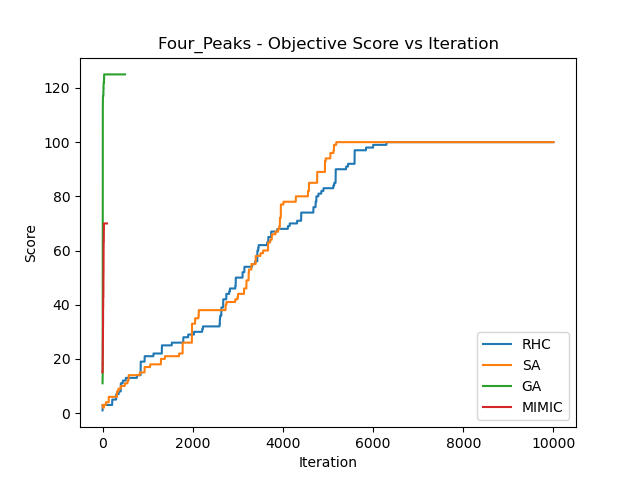
\includegraphics[width=0.70\textwidth]{../plots/Four_Peaks-ObjectiveVsIteration.png}}}
	\caption{Performance comparison for the Four Peaks problem. Lines represent the average score over each iteration when using different random state seeds. Shaded areas are the standard deviation.}
	\label{fig:fig1}
\end{figure}
% results table
\begin{center}
	\begin{tabular}{|c||c|c|c|}
	 \hline
	 Algorithm & Final Score & Average Runtime & Avg Time to Peak \\
	 \hline\hline
	 Random Hill Climb & 100 & 0.865s & 0.618s  \\
	 \hline
	 Simulated Annealing & 100 & 0.147s & 0.133s  \\
	 \hline
	 Genetic Algorithm & 189.0 & 32.992s & 8.791s  \\
	 \hline
	 MIMIC & 162.0 & 40.976s & 7.673s  \\
	 \hline
	\end{tabular}
	\label{table:table1}
\end{center}
As predicted, both random hill climbing and simulated annealing both settled in on suboptimal solutions, and genetic algorithm found the optimal fairly easily. Even though Simulated Annealing and Hill Climbing were orders of magnitude faster, it doesn't make much difference when the global optimals are never found. They could have run forever and never reached it. Throughout testing, there were some occasions when they got lucky, but most of the time, they settled on local maxima.

\subsubsection{Parameter Variation}
% parameter plots
\begin{figure}
	\centering
	\subfigure[]{\frame{\includegraphics[width=0.24\textwidth]{../plots/Four_Peaks-Random_Hill_Climbing_Over_restarts.png}}}
	\subfigure[]{\frame{\includegraphics[width=0.24\textwidth]{../plots/Four_Peaks-Simulated_Annealing_Over_decay_rate.png}}}
	\subfigure[]{\frame{\includegraphics[width=0.24\textwidth]{../plots/Four_Peaks-Genetic_Algorithm_Over_pop_size.png}}}
	\subfigure[]{\frame{\includegraphics[width=0.24\textwidth]{../plots/Four_Peaks-MIMIC_Over_pop_size.png}}}
	\caption{Parameter tuning for (a) RHC using number of random restarts, and (b) Simulated Annealing using rate of decay (c) GA using population size, and (d) MIMIC using population size}
	\label{fig:fig2}
\end{figure}
Iterating over a number of random restarts for the RHC algorithm shows expected results. There is basically a linear increase in runtime as restarts are increased, and it still doesn't help the end score. Hypothetically, with enough restarts, it would eventually find it, but that would be expensive.

Simulated Annealing doesn't fair much better. Changing the decay rate changes how quickly the algorithm settles on a solution. It shouldn't affect the runtime unless it finds a solution faster. Interestingly, there are a handful of configurations that are able to find the global optimal solution, but it seems to be mostly related to randomness, as there is no real trend.

Genetic Algorithm performs exceptionally well regardless of the population size. Since this is a relatively simple objective, that isn't too surprising. It also makes sense that runtime would scale linearly with increasing population.

MIMIC runtime scales linearly with population as well, but behaves strangely when it comes to the fitness score. Honestly, I can't really make sense of why there is no pattern. I would have expected fitness to improve with larger population since it would be able to gain more information about the probability densities and explore more of the problem space.

\subsection{Flip Flop}
\subsubsection{Theory and Prediction}
The Flip Flop problem is an interesting case because structure and relationships are important, which means that GA and MIMIC are likely to perform well, but it could still be captures using a gradient to some extent. Since what is most important is the relationship between parameters, and spacial information is relevant, I predict that MIMIC will perform the best, followed by GA, SA, then Random Hill climbing in last. MIMIC is especially good at capturing structure and relationship, and GA does this well too, but SA and RHC are not designed for this. The reason why I predict that SA will still perform relatively well is because it is designed to search the problem space more, so it is more likely to "accidentally" jump into a better solution.
\subsubsection{Performance}
% comparison graph
\begin{figure}
	\centering
	{\frame{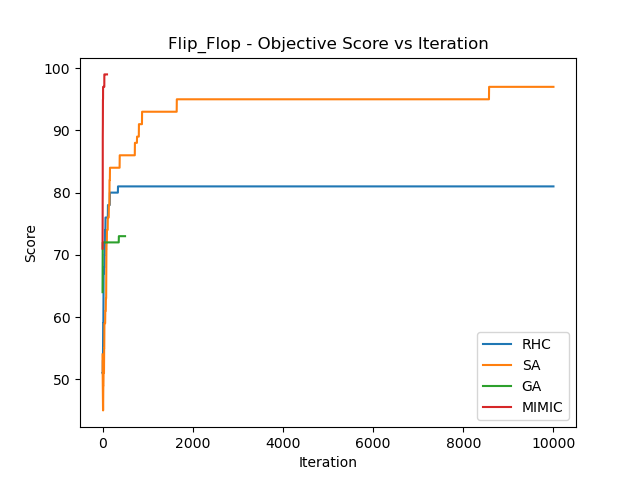
\includegraphics[width=0.70\textwidth]{../plots/Flip_Flop-ObjectiveVsIteration.png}}}
	\caption{Performance comparison for the Flip Flop problem. Lines represent the average score over each iteration when using different random state seeds. Shaded areas are the standard deviation.}
	\label{fig:fig3}
\end{figure}
% results table
\begin{center}
	\begin{tabular}{|c||c|c|c|}
	 \hline
	 Algorithm & Final Score & Average Runtime & Avg Time to Peak \\
	 \hline\hline
	 Random Hill Climb & 87 & 0.446s & 0.051s  \\
	 \hline
	 Simulated Annealing & 96 & 0.121s & 0.069s  \\
	 \hline
	 Genetic Algorithm & 95 & 39.87s & 7.93s  \\
	 \hline
	 MIMIC & 99 & 17.43s & 2.336s  \\
	 \hline
	\end{tabular}
	\label{table:table2}
\end{center}
Most of this is as predicted. MIMIC scores the best, but is also the slowest, and RHC is fast but does not perform well. The surprise here is how well Simulated Annealing has done. It has performed just barely better than GA, but much faster. Once again, it performs orders of magnitude faster than GA or MIMIC, and actually performs nearly just as well. Really the only algorithm not suited for this problem is RHC.

\subsubsection{Parameter Variation}
% param graphs
\begin{figure}
	\centering
	\subfigure[]{\frame{\includegraphics[width=0.24\textwidth]{../plots/Flip_Flop-Random_Hill_Climbing_Over_restarts.png}}}
	\subfigure[]{\frame{\includegraphics[width=0.24\textwidth]{../plots/Flip_Flop-Simulated_Annealing_Over_decay_rate.png}}}
	\subfigure[]{\frame{\includegraphics[width=0.24\textwidth]{../plots/Flip_Flop-Genetic_Algorithm_Over_pop_size.png}}}
	\subfigure[]{\frame{\includegraphics[width=0.24\textwidth]{../plots/Flip_Flop-MIMIC_Over_pop_size.png}}}
	\caption{Parameter tuning for (a) RHC using number of random restarts, and (b) Simulated Annealing using rate of decay (c) GA using population size, and (d) MIMIC using population size}
	\label{fig:fig4}
\end{figure}
Since random hill climbing requires luck to perform well in this situation, it's no surprise that increased restarts generally improve the fitness score, but it still plateaus since there is not a strong gradient to follow.

Just as with the last problem, Simulated Annealing is not affected much by the decay rate, at least not to where an obvious trend can be observed. There might a weak trend toward increasing fitness with increasing decay rate, but not enough to put much stock into it.

Genetic Algorithm improves with larger population, but it's a weak relationship since there are still dips. It is still surprising that it is weaker than the SA regardless of population. But just as before, larger population slows it down even more.

MIMIC is the only algorithm in this problem that has a very clear and obvious trend. As population size increases, so does the final accuracy. This is not surprising since it allows the algorithm to gain more information about the probability densities, and therefore make better predictions.

\subsection{Traveling Salesperson}
\subsubsection{Theory and Prediction}
The TSP (Traveling Salesperson Problem) involves iterating over many different paths in a large problem space. Because of the complexity of the problem, there are likely to be many local optimal solutions. Since there is a blend of a smooth objective function and significant structural or relational information, I predicted that MIMIC and GA will both reach more optimal solutions, but SA and RHC will reach suboptimal, but still very good solutions much faster.
\subsubsection{Performance}
% comparison graph
\begin{figure}
	\centering
	{\frame{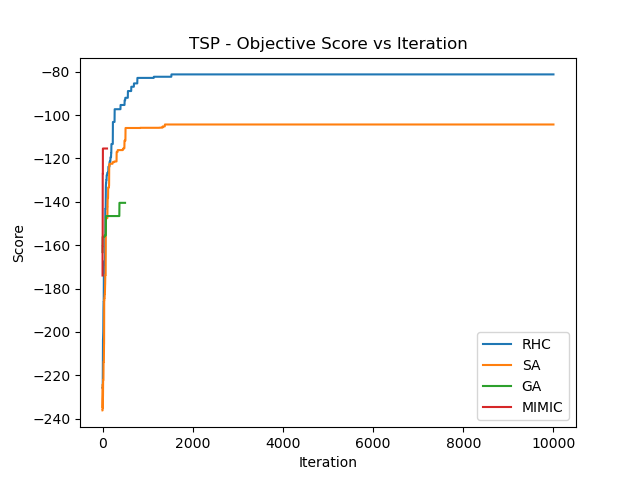
\includegraphics[width=0.70\textwidth]{../plots/TSP-ObjectiveVsIteration.png}}}
	\caption{Performance comparison for the Traveling Salesperson problem. Lines represent the average score over each iteration when using different random state seeds. Shaded areas are the standard deviation.}
	\label{fig:fig5}
\end{figure}
% results table
\begin{center}
	\begin{tabular}{|c||c|c|c|}
	 \hline
	 Algorithm & Final Score & Average Runtime & Avg Time to Peak \\
	 \hline\hline
	 Random Hill Climb & 102.2 & 1.121s & 2.80e-4s  \\
	 \hline
	 Simulated Annealing & 120.8 & 0.263s & 1.43e-4s  \\
	 \hline
	 Genetic Algorithm & 87.8 & 57.4s & 0.115s  \\
	 \hline
	 MIMIC & 133.2 & 238s & 0.952s  \\
	 \hline
	\end{tabular}
	\label{table:table3}
\end{center}
TSP definitely has the most surprising results compared to what I predicted. Basically the only thing I was correct about is that GA would be most accurate but slow, and SA/RHC would both be fast but suboptimal. However, I don't understand what happened to MIMIC and why it performed so poorly, nor do I understand why RHC was better than SA. Both of the gradient based algorithms are subject to chance regarding whether they would reach a global optimal, or something near the same value. They were much more likely to quickly settle on a local minimum, but I cant think of any reason why RHC would settle on a better solution than SA, since SA is more likely to explore more of the problem space. It could be related to tuning, but otherwise, it doesn't make much sense.

\subsubsection{Parameter Variation}
% param graphs
\begin{figure}
	\centering
	\subfigure[]{\frame{\includegraphics[width=0.24\textwidth]{../plots/TSP-Random_Hill_Climbing_Over_restarts.png}}}
	\subfigure[]{\frame{\includegraphics[width=0.24\textwidth]{../plots/TSP-Simulated_Annealing_Over_decay_rate.png}}}
	\subfigure[]{\frame{\includegraphics[width=0.24\textwidth]{../plots/TSP-Genetic_Algorithm_Over_pop_size.png}}}
	\subfigure[]{\frame{\includegraphics[width=0.24\textwidth]{../plots/TSP-MIMIC_Over_pop_size.png}}}
	\caption{Parameter tuning for (a) RHC using number of random restarts, and (b) Simulated Annealing using rate of decay (c) GA using population size, and (d) MIMIC using population size}
	\label{fig:fig6}
\end{figure}
Even though RHC compared to other algorithms was surprising, the parameter tuning was not. It has the same linear increase in runtime, and gets closer to optimal with more restarts.

Simulated Annealing is apparently very sensitive to how the TSP problem is designed. In this configuration used, setting the decay rate to 0.4 would have resulted in a much better solution, but no real trend otherwise. It seems that having a rate too low doesn't allow it to converge, and too high means it converges too soon. It's also likely that the optimal decay rate would change based on the parameters of the TSP.

Genetic Algorithm behaved exactly as expected. Since it can explore the problem space very well, it reaches an optimal solution with higher population. It is particularly well suited to this kind of problem.

MIMIC is similar to GA in that higher population increases end accuracy, but I'm still surprised that it was not able to reach an optimal solution, even at a pop size of 2000.

\section{Randomized Optimization in Neural Networks}
\subsection{Summary}
%TODO

%TODO

\section{Conclusion}
%TODO

\newpage

\section{References}
\nocite{Hayes19}
\nocite{Mitchell}
\nocite{Rollings20}
\printbibliography

\end{document}
